\documentclass[twoside]{book}

% Packages required by doxygen
\usepackage{fixltx2e}
\usepackage{calc}
\usepackage{doxygen}
\usepackage[export]{adjustbox} % also loads graphicx
\usepackage{graphicx}
\usepackage[utf8]{inputenc}
\usepackage{makeidx}
\usepackage{multicol}
\usepackage{multirow}
\PassOptionsToPackage{warn}{textcomp}
\usepackage{textcomp}
\usepackage[nointegrals]{wasysym}
\usepackage[table]{xcolor}

% Font selection
\usepackage[T1]{fontenc}
\usepackage[scaled=.90]{helvet}
\usepackage{courier}
\usepackage{amssymb}
\usepackage{sectsty}
\renewcommand{\familydefault}{\sfdefault}
\allsectionsfont{%
  \fontseries{bc}\selectfont%
  \color{darkgray}%
}
\renewcommand{\DoxyLabelFont}{%
  \fontseries{bc}\selectfont%
  \color{darkgray}%
}
\newcommand{\+}{\discretionary{\mbox{\scriptsize$\hookleftarrow$}}{}{}}

% Page & text layout
\usepackage{geometry}
\geometry{%
  a4paper,%
  top=2.5cm,%
  bottom=2.5cm,%
  left=2.5cm,%
  right=2.5cm%
}
\tolerance=750
\hfuzz=15pt
\hbadness=750
\setlength{\emergencystretch}{15pt}
\setlength{\parindent}{0cm}
\setlength{\parskip}{3ex plus 2ex minus 2ex}
\makeatletter
\renewcommand{\paragraph}{%
  \@startsection{paragraph}{4}{0ex}{-1.0ex}{1.0ex}{%
    \normalfont\normalsize\bfseries\SS@parafont%
  }%
}
\renewcommand{\subparagraph}{%
  \@startsection{subparagraph}{5}{0ex}{-1.0ex}{1.0ex}{%
    \normalfont\normalsize\bfseries\SS@subparafont%
  }%
}
\makeatother

% Headers & footers
\usepackage{fancyhdr}
\pagestyle{fancyplain}
\fancyhead[LE]{\fancyplain{}{\bfseries\thepage}}
\fancyhead[CE]{\fancyplain{}{}}
\fancyhead[RE]{\fancyplain{}{\bfseries\leftmark}}
\fancyhead[LO]{\fancyplain{}{\bfseries\rightmark}}
\fancyhead[CO]{\fancyplain{}{}}
\fancyhead[RO]{\fancyplain{}{\bfseries\thepage}}
\fancyfoot[LE]{\fancyplain{}{}}
\fancyfoot[CE]{\fancyplain{}{}}
\fancyfoot[RE]{\fancyplain{}{\bfseries\scriptsize Generated by Doxygen }}
\fancyfoot[LO]{\fancyplain{}{\bfseries\scriptsize Generated by Doxygen }}
\fancyfoot[CO]{\fancyplain{}{}}
\fancyfoot[RO]{\fancyplain{}{}}
\renewcommand{\footrulewidth}{0.4pt}
\renewcommand{\chaptermark}[1]{%
  \markboth{#1}{}%
}
\renewcommand{\sectionmark}[1]{%
  \markright{\thesection\ #1}%
}

% Indices & bibliography
\usepackage{natbib}
\usepackage[titles]{tocloft}
\setcounter{tocdepth}{3}
\setcounter{secnumdepth}{5}
\makeindex

% Hyperlinks (required, but should be loaded last)
\usepackage{ifpdf}
\ifpdf
  \usepackage[pdftex,pagebackref=true]{hyperref}
\else
  \usepackage[ps2pdf,pagebackref=true]{hyperref}
\fi
\hypersetup{%
  colorlinks=true,%
  linkcolor=blue,%
  citecolor=blue,%
  unicode%
}

% Custom commands
\newcommand{\clearemptydoublepage}{%
  \newpage{\pagestyle{empty}\cleardoublepage}%
}

\usepackage{caption}
\captionsetup{labelsep=space,justification=centering,font={bf},singlelinecheck=off,skip=4pt,position=top}

%===== C O N T E N T S =====

\begin{document}

% Titlepage & ToC
\hypersetup{pageanchor=false,
             bookmarksnumbered=true,
             pdfencoding=unicode
            }
\pagenumbering{roman}
\begin{titlepage}
\vspace*{7cm}
\begin{center}%
{\Large My Project }\\
\vspace*{1cm}
{\large Generated by Doxygen 1.8.11}\\
\end{center}
\end{titlepage}
\clearemptydoublepage
\tableofcontents
\clearemptydoublepage
\pagenumbering{arabic}
\hypersetup{pageanchor=true}

%--- Begin generated contents ---
\chapter{Class Index}
\section{Class List}
Here are the classes, structs, unions and interfaces with brief descriptions\+:\begin{DoxyCompactList}
\item\contentsline{section}{\hyperlink{structarena}{arena} }{\pageref{structarena}}{}
\item\contentsline{section}{\hyperlink{structblock}{block} }{\pageref{structblock}}{}
\item\contentsline{section}{\hyperlink{structcondition}{condition} }{\pageref{structcondition}}{}
\item\contentsline{section}{\hyperlink{structdesc}{desc} }{\pageref{structdesc}}{}
\item\contentsline{section}{\hyperlink{structintr__frame}{intr\+\_\+frame} }{\pageref{structintr__frame}}{}
\item\contentsline{section}{\hyperlink{structkernel__thread__frame}{kernel\+\_\+thread\+\_\+frame} }{\pageref{structkernel__thread__frame}}{}
\item\contentsline{section}{\hyperlink{structlock}{lock} }{\pageref{structlock}}{}
\item\contentsline{section}{\hyperlink{structpool}{pool} }{\pageref{structpool}}{}
\item\contentsline{section}{\hyperlink{structsemaphore}{semaphore} }{\pageref{structsemaphore}}{}
\item\contentsline{section}{\hyperlink{structsemaphore__elem}{semaphore\+\_\+elem} }{\pageref{structsemaphore__elem}}{}
\item\contentsline{section}{\hyperlink{structswitch__entry__frame}{switch\+\_\+entry\+\_\+frame} }{\pageref{structswitch__entry__frame}}{}
\item\contentsline{section}{\hyperlink{structswitch__threads__frame}{switch\+\_\+threads\+\_\+frame} }{\pageref{structswitch__threads__frame}}{}
\item\contentsline{section}{\hyperlink{structthread}{thread} }{\pageref{structthread}}{}
\end{DoxyCompactList}

\chapter{File Index}
\section{File List}
Here is a list of all documented files with brief descriptions\+:\begin{DoxyCompactList}
\item\contentsline{section}{{\bfseries flags.\+h} }{\pageref{flags_8h}}{}
\item\contentsline{section}{{\bfseries init.\+h} }{\pageref{init_8h}}{}
\item\contentsline{section}{{\bfseries interrupt.\+h} }{\pageref{interrupt_8h}}{}
\item\contentsline{section}{{\bfseries intr-\/stubs.\+h} }{\pageref{intr-stubs_8h}}{}
\item\contentsline{section}{{\bfseries io.\+h} }{\pageref{io_8h}}{}
\item\contentsline{section}{{\bfseries loader.\+h} }{\pageref{loader_8h}}{}
\item\contentsline{section}{{\bfseries malloc.\+h} }{\pageref{malloc_8h}}{}
\item\contentsline{section}{{\bfseries palloc.\+h} }{\pageref{palloc_8h}}{}
\item\contentsline{section}{{\bfseries pte.\+h} }{\pageref{pte_8h}}{}
\item\contentsline{section}{\hyperlink{shell_8c}{shell.\+c} \\*Implementacion de un shell para Pintos }{\pageref{shell_8c}}{}
\item\contentsline{section}{{\bfseries switch.\+h} }{\pageref{switch_8h}}{}
\item\contentsline{section}{{\bfseries synch.\+h} }{\pageref{synch_8h}}{}
\item\contentsline{section}{{\bfseries thread.\+h} }{\pageref{thread_8h}}{}
\item\contentsline{section}{{\bfseries vaddr.\+h} }{\pageref{vaddr_8h}}{}
\end{DoxyCompactList}

\chapter{Class Documentation}
\hypertarget{structarena}{}\section{arena Struct Reference}
\label{structarena}\index{arena@{arena}}


Collaboration diagram for arena\+:
\nopagebreak
\begin{figure}[H]
\begin{center}
\leavevmode
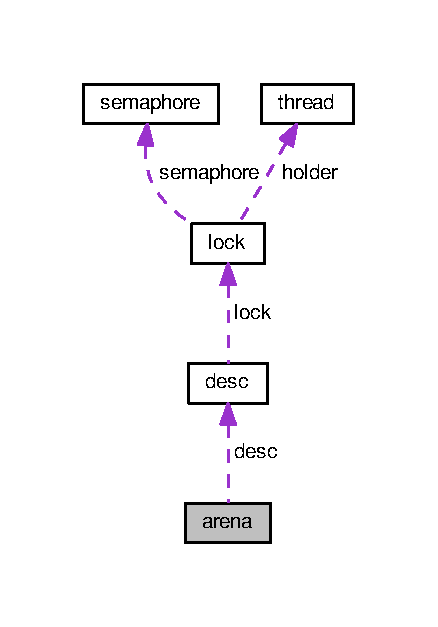
\includegraphics[width=210pt]{structarena__coll__graph}
\end{center}
\end{figure}
\subsection*{Public Attributes}
\begin{DoxyCompactItemize}
\item 
unsigned {\bfseries magic}\hypertarget{structarena_a46406b9b6a981618886e52962d6afc37}{}\label{structarena_a46406b9b6a981618886e52962d6afc37}

\item 
struct \hyperlink{structdesc}{desc} $\ast$ {\bfseries desc}\hypertarget{structarena_abe94de22726d93178a59e0278000b070}{}\label{structarena_abe94de22726d93178a59e0278000b070}

\item 
size\+\_\+t {\bfseries free\+\_\+cnt}\hypertarget{structarena_a42d04c18c83b0289c75c6c429d1ae566}{}\label{structarena_a42d04c18c83b0289c75c6c429d1ae566}

\end{DoxyCompactItemize}


The documentation for this struct was generated from the following file\+:\begin{DoxyCompactItemize}
\item 
malloc.\+c\end{DoxyCompactItemize}

\hypertarget{structblock}{}\section{block Struct Reference}
\label{structblock}\index{block@{block}}
\subsection*{Public Attributes}
\begin{DoxyCompactItemize}
\item 
struct list\+\_\+elem {\bfseries free\+\_\+elem}\hypertarget{structblock_aeb1e367fcd8d93b045459618add975d2}{}\label{structblock_aeb1e367fcd8d93b045459618add975d2}

\end{DoxyCompactItemize}


The documentation for this struct was generated from the following file\+:\begin{DoxyCompactItemize}
\item 
malloc.\+c\end{DoxyCompactItemize}

\hypertarget{structcondition}{}\section{condition Struct Reference}
\label{structcondition}\index{condition@{condition}}
\subsection*{Public Attributes}
\begin{DoxyCompactItemize}
\item 
struct list {\bfseries waiters}\hypertarget{structcondition_a85e047c99fb328f32b7e61c9565d1ca7}{}\label{structcondition_a85e047c99fb328f32b7e61c9565d1ca7}

\end{DoxyCompactItemize}


The documentation for this struct was generated from the following file\+:\begin{DoxyCompactItemize}
\item 
synch.\+h\end{DoxyCompactItemize}

\hypertarget{structdesc}{}\section{desc Struct Reference}
\label{structdesc}\index{desc@{desc}}


Collaboration diagram for desc\+:
\nopagebreak
\begin{figure}[H]
\begin{center}
\leavevmode
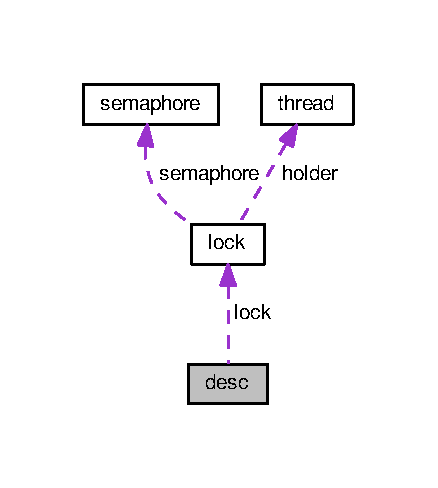
\includegraphics[width=210pt]{structdesc__coll__graph}
\end{center}
\end{figure}
\subsection*{Public Attributes}
\begin{DoxyCompactItemize}
\item 
size\+\_\+t {\bfseries block\+\_\+size}\hypertarget{structdesc_a069c5d50b953f029c330020ca4735731}{}\label{structdesc_a069c5d50b953f029c330020ca4735731}

\item 
size\+\_\+t {\bfseries blocks\+\_\+per\+\_\+arena}\hypertarget{structdesc_ade728d0cc6c3b71571e8aaf4301863e2}{}\label{structdesc_ade728d0cc6c3b71571e8aaf4301863e2}

\item 
struct list {\bfseries free\+\_\+list}\hypertarget{structdesc_a0b6c63f462b9c00a0241d03ea05b192e}{}\label{structdesc_a0b6c63f462b9c00a0241d03ea05b192e}

\item 
struct \hyperlink{structlock}{lock} {\bfseries lock}\hypertarget{structdesc_a3f87cf0070aa73d4d9739648a217992b}{}\label{structdesc_a3f87cf0070aa73d4d9739648a217992b}

\end{DoxyCompactItemize}


The documentation for this struct was generated from the following file\+:\begin{DoxyCompactItemize}
\item 
malloc.\+c\end{DoxyCompactItemize}

\hypertarget{structintr__frame}{}\section{intr\+\_\+frame Struct Reference}
\label{structintr__frame}\index{intr\+\_\+frame@{intr\+\_\+frame}}
\subsection*{Public Attributes}
\begin{DoxyCompactItemize}
\item 
uint32\+\_\+t {\bfseries edi}\hypertarget{structintr__frame_ac7dcd3ff5e0eadd92d3e998fce6c83cc}{}\label{structintr__frame_ac7dcd3ff5e0eadd92d3e998fce6c83cc}

\item 
uint32\+\_\+t {\bfseries esi}\hypertarget{structintr__frame_ade7a4007ee748b10ca2ad37c94f89ef2}{}\label{structintr__frame_ade7a4007ee748b10ca2ad37c94f89ef2}

\item 
uint32\+\_\+t {\bfseries ebp}\hypertarget{structintr__frame_aca6b77168c58177683f839a31c9499d3}{}\label{structintr__frame_aca6b77168c58177683f839a31c9499d3}

\item 
uint32\+\_\+t {\bfseries esp\+\_\+dummy}\hypertarget{structintr__frame_a53c788aace1f6e8dce31a0c1b8e5efbd}{}\label{structintr__frame_a53c788aace1f6e8dce31a0c1b8e5efbd}

\item 
uint32\+\_\+t {\bfseries ebx}\hypertarget{structintr__frame_a5836123b995e4f029df26009ad2e32bb}{}\label{structintr__frame_a5836123b995e4f029df26009ad2e32bb}

\item 
uint32\+\_\+t {\bfseries edx}\hypertarget{structintr__frame_ab3e46e99e78343016ebfc2db8d2bab4c}{}\label{structintr__frame_ab3e46e99e78343016ebfc2db8d2bab4c}

\item 
uint32\+\_\+t {\bfseries ecx}\hypertarget{structintr__frame_ab2c4de68744ed3116cf89cc90f840ee0}{}\label{structintr__frame_ab2c4de68744ed3116cf89cc90f840ee0}

\item 
uint32\+\_\+t {\bfseries eax}\hypertarget{structintr__frame_aca38582b8d9a281dcf21ee0e064ad615}{}\label{structintr__frame_aca38582b8d9a281dcf21ee0e064ad615}

\item 
uint16\+\_\+t {\bfseries gs}\hypertarget{structintr__frame_ac0acccfad5d77495802651d27d2e729f}{}\label{structintr__frame_ac0acccfad5d77495802651d27d2e729f}

\item 
uint16\+\_\+t uint16\+\_\+t {\bfseries fs}\+:16\hypertarget{structintr__frame_a4967c5b3c4ee2ba8161c867d7ba5c9ef}{}\label{structintr__frame_a4967c5b3c4ee2ba8161c867d7ba5c9ef}

\item 
uint16\+\_\+t uint16\+\_\+t uint16\+\_\+t {\bfseries es}\+:16\hypertarget{structintr__frame_a9c32903d5d6a0e5f23d167fdc75b057a}{}\label{structintr__frame_a9c32903d5d6a0e5f23d167fdc75b057a}

\item 
uint16\+\_\+t uint16\+\_\+t uint16\+\_\+t uint16\+\_\+t {\bfseries ds}\+:16\hypertarget{structintr__frame_a9fc5e5d66dbc18aed5360cf2973289da}{}\label{structintr__frame_a9fc5e5d66dbc18aed5360cf2973289da}

\item 
uint16\+\_\+t uint16\+\_\+t uint16\+\_\+t uint16\+\_\+t uint32\+\_\+t {\bfseries vec\+\_\+no}\+:16\hypertarget{structintr__frame_a5220184751c984a6ad28d14ef43183e3}{}\label{structintr__frame_a5220184751c984a6ad28d14ef43183e3}

\item 
uint32\+\_\+t {\bfseries error\+\_\+code}\hypertarget{structintr__frame_a54168d3e26b008b0fc15e033ee76630a}{}\label{structintr__frame_a54168d3e26b008b0fc15e033ee76630a}

\item 
void $\ast$ {\bfseries frame\+\_\+pointer}\hypertarget{structintr__frame_a1b89f0706f01818a1e88cd36b41e8a47}{}\label{structintr__frame_a1b89f0706f01818a1e88cd36b41e8a47}

\item 
void($\ast$ {\bfseries eip} )(void)\hypertarget{structintr__frame_a45b946407a784749cf08cf9144f3b980}{}\label{structintr__frame_a45b946407a784749cf08cf9144f3b980}

\item 
uint16\+\_\+t {\bfseries cs}\hypertarget{structintr__frame_adc947ba61eb2eee7f5a01252fd271e09}{}\label{structintr__frame_adc947ba61eb2eee7f5a01252fd271e09}

\item 
uint16\+\_\+t uint32\+\_\+t {\bfseries eflags}\+:16\hypertarget{structintr__frame_a20b094789ff3ccc8f0f1fa5a7e350491}{}\label{structintr__frame_a20b094789ff3ccc8f0f1fa5a7e350491}

\item 
void $\ast$ {\bfseries esp}\hypertarget{structintr__frame_ac0f61c482c6dee39e39ec3f28833f595}{}\label{structintr__frame_ac0f61c482c6dee39e39ec3f28833f595}

\item 
uint16\+\_\+t {\bfseries ss}\hypertarget{structintr__frame_a27f574cac8439151d57354d344259f57}{}\label{structintr__frame_a27f574cac8439151d57354d344259f57}

\end{DoxyCompactItemize}


The documentation for this struct was generated from the following file\+:\begin{DoxyCompactItemize}
\item 
interrupt.\+h\end{DoxyCompactItemize}

\hypertarget{structkernel__thread__frame}{}\section{kernel\+\_\+thread\+\_\+frame Struct Reference}
\label{structkernel__thread__frame}\index{kernel\+\_\+thread\+\_\+frame@{kernel\+\_\+thread\+\_\+frame}}
\subsection*{Public Attributes}
\begin{DoxyCompactItemize}
\item 
void $\ast$ {\bfseries eip}\hypertarget{structkernel__thread__frame_ad09a36aad7e8ab228235d49f0975edf4}{}\label{structkernel__thread__frame_ad09a36aad7e8ab228235d49f0975edf4}

\item 
thread\+\_\+func $\ast$ {\bfseries function}\hypertarget{structkernel__thread__frame_ab291ec9659556df6e215dc2d1201515b}{}\label{structkernel__thread__frame_ab291ec9659556df6e215dc2d1201515b}

\item 
void $\ast$ {\bfseries aux}\hypertarget{structkernel__thread__frame_a6bcf2dfdd3a5803ce9dd714e1690c200}{}\label{structkernel__thread__frame_a6bcf2dfdd3a5803ce9dd714e1690c200}

\end{DoxyCompactItemize}


The documentation for this struct was generated from the following file\+:\begin{DoxyCompactItemize}
\item 
thread.\+c\end{DoxyCompactItemize}

\hypertarget{structlock}{}\section{lock Struct Reference}
\label{structlock}\index{lock@{lock}}


Collaboration diagram for lock\+:
\nopagebreak
\begin{figure}[H]
\begin{center}
\leavevmode
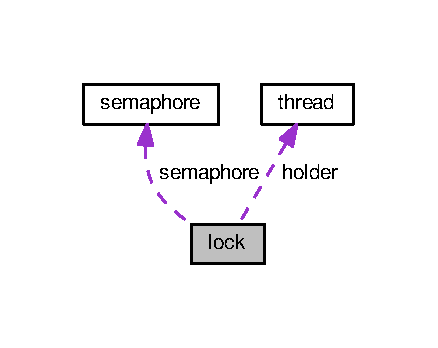
\includegraphics[width=210pt]{structlock__coll__graph}
\end{center}
\end{figure}
\subsection*{Public Attributes}
\begin{DoxyCompactItemize}
\item 
struct \hyperlink{structthread}{thread} $\ast$ {\bfseries holder}\hypertarget{structlock_a810cc844d1cb512db077a531b5310c6c}{}\label{structlock_a810cc844d1cb512db077a531b5310c6c}

\item 
struct \hyperlink{structsemaphore}{semaphore} {\bfseries semaphore}\hypertarget{structlock_abb2cd5e8ae70282e2d1b584f347dc9f3}{}\label{structlock_abb2cd5e8ae70282e2d1b584f347dc9f3}

\end{DoxyCompactItemize}


The documentation for this struct was generated from the following file\+:\begin{DoxyCompactItemize}
\item 
synch.\+h\end{DoxyCompactItemize}

\hypertarget{structpool}{}\section{pool Struct Reference}
\label{structpool}\index{pool@{pool}}


Collaboration diagram for pool\+:
\nopagebreak
\begin{figure}[H]
\begin{center}
\leavevmode
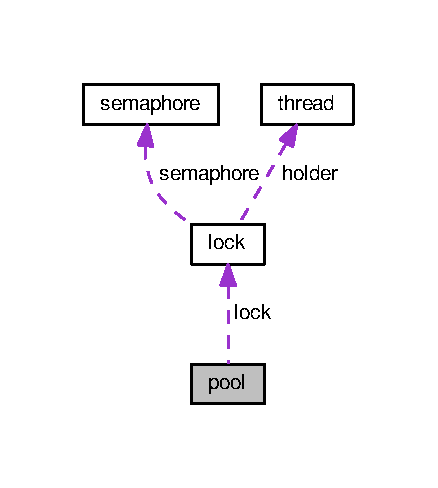
\includegraphics[width=210pt]{structpool__coll__graph}
\end{center}
\end{figure}
\subsection*{Public Attributes}
\begin{DoxyCompactItemize}
\item 
struct \hyperlink{structlock}{lock} {\bfseries lock}\hypertarget{structpool_ae9331ff5a685b586cd3693b68daf5b4f}{}\label{structpool_ae9331ff5a685b586cd3693b68daf5b4f}

\item 
struct bitmap $\ast$ {\bfseries used\+\_\+map}\hypertarget{structpool_a2466db5ef7583841658d26d5ccfab9a1}{}\label{structpool_a2466db5ef7583841658d26d5ccfab9a1}

\item 
uint8\+\_\+t $\ast$ {\bfseries base}\hypertarget{structpool_aab1398419a45bb23a0e617a50e7dc1fb}{}\label{structpool_aab1398419a45bb23a0e617a50e7dc1fb}

\end{DoxyCompactItemize}


The documentation for this struct was generated from the following file\+:\begin{DoxyCompactItemize}
\item 
palloc.\+c\end{DoxyCompactItemize}

\hypertarget{structsemaphore}{}\section{semaphore Struct Reference}
\label{structsemaphore}\index{semaphore@{semaphore}}
\subsection*{Public Attributes}
\begin{DoxyCompactItemize}
\item 
unsigned {\bfseries value}\hypertarget{structsemaphore_a0b69d8b576949ef9277c3231e09fd3c6}{}\label{structsemaphore_a0b69d8b576949ef9277c3231e09fd3c6}

\item 
struct list {\bfseries waiters}\hypertarget{structsemaphore_a256e316ba2f3f9b59497f109cf0daee5}{}\label{structsemaphore_a256e316ba2f3f9b59497f109cf0daee5}

\end{DoxyCompactItemize}


The documentation for this struct was generated from the following file\+:\begin{DoxyCompactItemize}
\item 
synch.\+h\end{DoxyCompactItemize}

\hypertarget{structsemaphore__elem}{}\section{semaphore\+\_\+elem Struct Reference}
\label{structsemaphore__elem}\index{semaphore\+\_\+elem@{semaphore\+\_\+elem}}


Collaboration diagram for semaphore\+\_\+elem\+:
\nopagebreak
\begin{figure}[H]
\begin{center}
\leavevmode
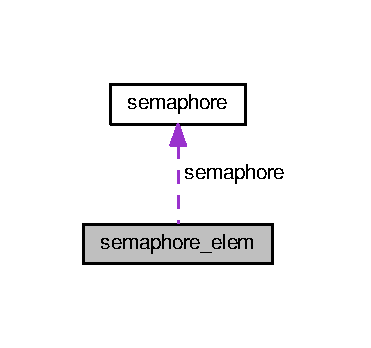
\includegraphics[width=178pt]{structsemaphore__elem__coll__graph}
\end{center}
\end{figure}
\subsection*{Public Attributes}
\begin{DoxyCompactItemize}
\item 
struct list\+\_\+elem {\bfseries elem}\hypertarget{structsemaphore__elem_a1156a1cac7fcbc1447b40867da1ce406}{}\label{structsemaphore__elem_a1156a1cac7fcbc1447b40867da1ce406}

\item 
struct \hyperlink{structsemaphore}{semaphore} {\bfseries semaphore}\hypertarget{structsemaphore__elem_af1b97cc65c3aabff2f3da9335e3784a9}{}\label{structsemaphore__elem_af1b97cc65c3aabff2f3da9335e3784a9}

\end{DoxyCompactItemize}


The documentation for this struct was generated from the following file\+:\begin{DoxyCompactItemize}
\item 
synch.\+c\end{DoxyCompactItemize}

\hypertarget{structswitch__entry__frame}{}\section{switch\+\_\+entry\+\_\+frame Struct Reference}
\label{structswitch__entry__frame}\index{switch\+\_\+entry\+\_\+frame@{switch\+\_\+entry\+\_\+frame}}
\subsection*{Public Attributes}
\begin{DoxyCompactItemize}
\item 
void($\ast$ {\bfseries eip} )(void)\hypertarget{structswitch__entry__frame_a521611ca37058e2aed783fa7ca7bd6b9}{}\label{structswitch__entry__frame_a521611ca37058e2aed783fa7ca7bd6b9}

\end{DoxyCompactItemize}


The documentation for this struct was generated from the following file\+:\begin{DoxyCompactItemize}
\item 
switch.\+h\end{DoxyCompactItemize}

\hypertarget{structswitch__threads__frame}{}\section{switch\+\_\+threads\+\_\+frame Struct Reference}
\label{structswitch__threads__frame}\index{switch\+\_\+threads\+\_\+frame@{switch\+\_\+threads\+\_\+frame}}


Collaboration diagram for switch\+\_\+threads\+\_\+frame\+:
\nopagebreak
\begin{figure}[H]
\begin{center}
\leavevmode
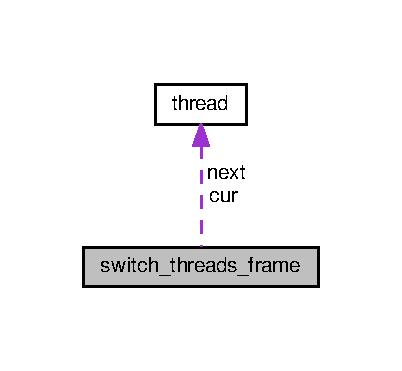
\includegraphics[width=193pt]{structswitch__threads__frame__coll__graph}
\end{center}
\end{figure}
\subsection*{Public Attributes}
\begin{DoxyCompactItemize}
\item 
uint32\+\_\+t {\bfseries edi}\hypertarget{structswitch__threads__frame_a4f8ccb09ef3e05eae1d9442cf2803b14}{}\label{structswitch__threads__frame_a4f8ccb09ef3e05eae1d9442cf2803b14}

\item 
uint32\+\_\+t {\bfseries esi}\hypertarget{structswitch__threads__frame_accf719c0384f6832ab3299fe524168b0}{}\label{structswitch__threads__frame_accf719c0384f6832ab3299fe524168b0}

\item 
uint32\+\_\+t {\bfseries ebp}\hypertarget{structswitch__threads__frame_a4097c9b97cf2e2a06d5315b9c7cab2a2}{}\label{structswitch__threads__frame_a4097c9b97cf2e2a06d5315b9c7cab2a2}

\item 
uint32\+\_\+t {\bfseries ebx}\hypertarget{structswitch__threads__frame_ac3b0ed0a688fa3aae89c0f50550e1c76}{}\label{structswitch__threads__frame_ac3b0ed0a688fa3aae89c0f50550e1c76}

\item 
void($\ast$ {\bfseries eip} )(void)\hypertarget{structswitch__threads__frame_a03417cf6abfc21346097ef4a9fcc5185}{}\label{structswitch__threads__frame_a03417cf6abfc21346097ef4a9fcc5185}

\item 
struct \hyperlink{structthread}{thread} $\ast$ {\bfseries cur}\hypertarget{structswitch__threads__frame_a356ecdfdd2fcc59857cab85b1f2b4266}{}\label{structswitch__threads__frame_a356ecdfdd2fcc59857cab85b1f2b4266}

\item 
struct \hyperlink{structthread}{thread} $\ast$ {\bfseries next}\hypertarget{structswitch__threads__frame_a061c58993096523ce860e859e0706c79}{}\label{structswitch__threads__frame_a061c58993096523ce860e859e0706c79}

\end{DoxyCompactItemize}


The documentation for this struct was generated from the following file\+:\begin{DoxyCompactItemize}
\item 
switch.\+h\end{DoxyCompactItemize}

\hypertarget{structthread}{}\section{thread Struct Reference}
\label{structthread}\index{thread@{thread}}
\subsection*{Public Attributes}
\begin{DoxyCompactItemize}
\item 
tid\+\_\+t {\bfseries tid}\hypertarget{structthread_a7360cfa969a95354a5756946205b1138}{}\label{structthread_a7360cfa969a95354a5756946205b1138}

\item 
enum thread\+\_\+status {\bfseries status}\hypertarget{structthread_ac0b66a487cfb69469a807077cd801290}{}\label{structthread_ac0b66a487cfb69469a807077cd801290}

\item 
char {\bfseries name} \mbox{[}16\mbox{]}\hypertarget{structthread_a59ebdca51eb8eabddbe6d26b4c13c3ab}{}\label{structthread_a59ebdca51eb8eabddbe6d26b4c13c3ab}

\item 
uint8\+\_\+t $\ast$ {\bfseries stack}\hypertarget{structthread_a13be198956c306ad7f4ab1de2a91df73}{}\label{structthread_a13be198956c306ad7f4ab1de2a91df73}

\item 
int {\bfseries priority}\hypertarget{structthread_a04d1040ba1acd5961797345743567293}{}\label{structthread_a04d1040ba1acd5961797345743567293}

\item 
struct list\+\_\+elem {\bfseries allelem}\hypertarget{structthread_a21b7f77466e0383cc9dd51988ea131d6}{}\label{structthread_a21b7f77466e0383cc9dd51988ea131d6}

\item 
struct list\+\_\+elem {\bfseries elem}\hypertarget{structthread_a4542f0a9644fb012de20399c8e15c741}{}\label{structthread_a4542f0a9644fb012de20399c8e15c741}

\item 
unsigned {\bfseries magic}\hypertarget{structthread_a3a49980d160800cda815248d91e47052}{}\label{structthread_a3a49980d160800cda815248d91e47052}

\end{DoxyCompactItemize}


The documentation for this struct was generated from the following file\+:\begin{DoxyCompactItemize}
\item 
thread.\+h\end{DoxyCompactItemize}

\chapter{File Documentation}
\hypertarget{shell_8c}{}\section{shell.\+c File Reference}
\label{shell_8c}\index{shell.\+c@{shell.\+c}}


Implementacion de un shell para Pintos.  


{\ttfamily \#include \char`\"{}lib/stdio.\+h\char`\"{}}\\*
{\ttfamily \#include \char`\"{}kernel/console.\+h\char`\"{}}\\*
{\ttfamily \#include \char`\"{}lib/stdlib.\+h\char`\"{}}\\*
{\ttfamily \#include \char`\"{}devices/input.\+h\char`\"{}}\\*
{\ttfamily \#include \char`\"{}lib/string.\+h\char`\"{}}\\*
{\ttfamily \#include $<$stdbool.\+h$>$}\\*
{\ttfamily \#include $<$stddef.\+h$>$}\\*
{\ttfamily \#include $<$stdint.\+h$>$}\\*
{\ttfamily \#include \char`\"{}filesys/file.\+h\char`\"{}}\\*
{\ttfamily \#include \char`\"{}filesys/filesys.\+h\char`\"{}}\\*
Include dependency graph for shell.\+c\+:
\nopagebreak
\begin{figure}[H]
\begin{center}
\leavevmode
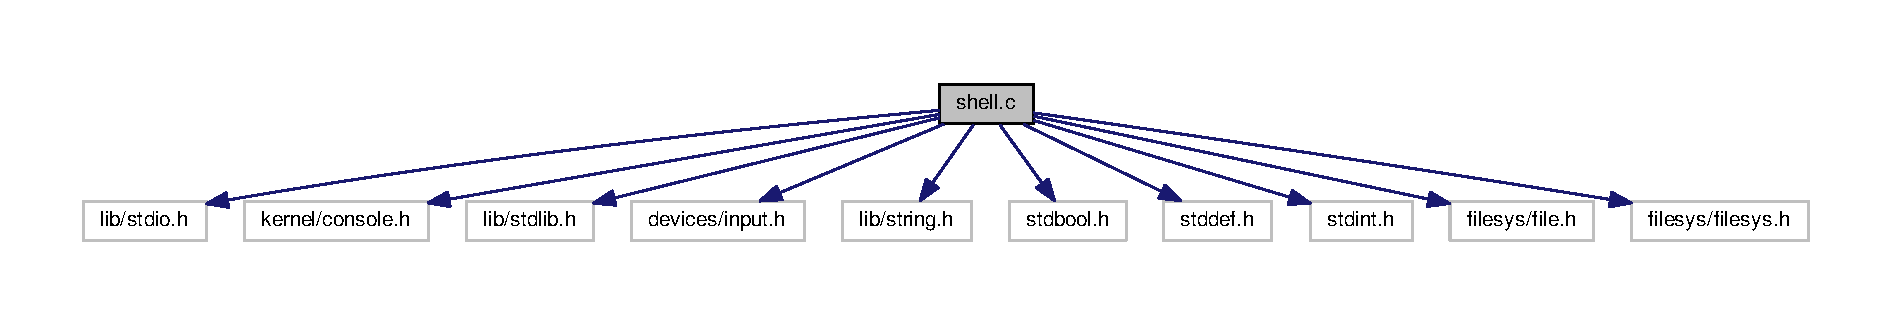
\includegraphics[width=350pt]{shell_8c__incl}
\end{center}
\end{figure}
\subsection*{Macros}
\begin{DoxyCompactItemize}
\item 
\#define {\bfseries I\+N\+P\+U\+T\+\_\+\+S\+I\+ZE}~50\hypertarget{shell_8c_abcf72cd23bdafb47b19023d91b4c107d}{}\label{shell_8c_abcf72cd23bdafb47b19023d91b4c107d}

\item 
\#define {\bfseries C\+A\+R\+R\+I\+A\+G\+E\+\_\+\+R\+E\+T\+U\+R\+N\+\_\+\+C\+H\+AR}~13\hypertarget{shell_8c_abdf9f7e5da7e68dcf6243ea1878e90cb}{}\label{shell_8c_abdf9f7e5da7e68dcf6243ea1878e90cb}

\item 
\#define {\bfseries M\+A\+T\+C\+H\+\_\+\+S\+U\+C\+C\+E\+SS}~0\hypertarget{shell_8c_a5f48dcc6eee4e04499a8b2a5e8f56b91}{}\label{shell_8c_a5f48dcc6eee4e04499a8b2a5e8f56b91}

\item 
\#define {\bfseries F\+I\+L\+E\+\_\+\+S\+I\+ZE}~40960\hypertarget{shell_8c_af3c3df6c9906ede8f09fa2af74cb28d5}{}\label{shell_8c_af3c3df6c9906ede8f09fa2af74cb28d5}

\end{DoxyCompactItemize}
\subsection*{Functions}
\begin{DoxyCompactItemize}
\item 
void {\bfseries remove\+\_\+file\+\_\+verbose} (char $\ast$)\hypertarget{shell_8c_a3a968be446f0e323bb03169935af55e7}{}\label{shell_8c_a3a968be446f0e323bb03169935af55e7}

\item 
void {\bfseries remove\+\_\+file} (char $\ast$)\hypertarget{shell_8c_ab7fadac0c9f8aa3dc91be6424599fae7}{}\label{shell_8c_ab7fadac0c9f8aa3dc91be6424599fae7}

\item 
bool {\bfseries rename\+\_\+file} (char $\ast$, char $\ast$)\hypertarget{shell_8c_a51ee302d9948b78206f91696fde08de9}{}\label{shell_8c_a51ee302d9948b78206f91696fde08de9}

\item 
int \hyperlink{shell_8c_a9f962247d6fee21d014cf0c334c6f99a}{shell} ()
\item 
void {\bfseries print\+\_\+rm\+\_\+help\+\_\+info} ()\hypertarget{shell_8c_a10501db4b9cca7d06b0c9272812732f5}{}\label{shell_8c_a10501db4b9cca7d06b0c9272812732f5}

\item 
void {\bfseries printf\+\_\+rm\+\_\+version\+\_\+info} ()\hypertarget{shell_8c_af47a51b5cf78dc987bf4bb189ac35ef9}{}\label{shell_8c_af47a51b5cf78dc987bf4bb189ac35ef9}

\item 
void {\bfseries printf\+\_\+mv\+\_\+help\+\_\+info} ()\hypertarget{shell_8c_adf163c66ec2d99650927b62c6d5d6101}{}\label{shell_8c_adf163c66ec2d99650927b62c6d5d6101}

\item 
void {\bfseries print\+\_\+mv\+\_\+version\+\_\+info} ()\hypertarget{shell_8c_aa9981a3f0fb531192f9344becbbdfbf5}{}\label{shell_8c_aa9981a3f0fb531192f9344becbbdfbf5}

\end{DoxyCompactItemize}
\subsection*{Variables}
\begin{DoxyCompactItemize}
\item 
char {\bfseries username} \mbox{[}$\,$\mbox{]} = \char`\"{}Ivan Valette\char`\"{}\hypertarget{shell_8c_aeb925e5210b37c37e0f03bafe4993550}{}\label{shell_8c_aeb925e5210b37c37e0f03bafe4993550}

\end{DoxyCompactItemize}


\subsection{Detailed Description}
Implementacion de un shell para Pintos. 

\begin{DoxyAuthor}{Author}
Ivan Valette 
\end{DoxyAuthor}


\subsection{Function Documentation}
\index{shell.\+c@{shell.\+c}!shell@{shell}}
\index{shell@{shell}!shell.\+c@{shell.\+c}}
\subsubsection[{\texorpdfstring{shell()}{shell()}}]{\setlength{\rightskip}{0pt plus 5cm}int shell (
\begin{DoxyParamCaption}
{}
\end{DoxyParamCaption}
)}\hypertarget{shell_8c_a9f962247d6fee21d014cf0c334c6f99a}{}\label{shell_8c_a9f962247d6fee21d014cf0c334c6f99a}
Shell para Pintos capaz de reconocer los comandos whoami\+: imprime el nombre del usuario en consola exit\+: concluye el shell y permite que Pintos termine

En caso de que se teclee un comando diferente a los descritos anteriormente se informara al usuario que el comando es desconocido. 
%--- End generated contents ---

% Index
\backmatter
\newpage
\phantomsection
\clearemptydoublepage
\addcontentsline{toc}{chapter}{Index}
\printindex

\end{document}
